\documentclass[12pt]{article}
\usepackage{../../../lecture_notes}
\usepackage{../../../math}
\usepackage{../../../uark_colors}

\hypersetup{
  colorlinks = true,
  allcolors = ozark_mountains,
  breaklinks = true,
  bookmarksopen = true
}

\begin{document}
\begin{center}
  {\Huge\bf Midterm 2 - Fall 2024}
  
  \smallskip
  {\large\it  ECON 4753 — University of Arkansas}
\end{center}

\vspace{5mm}
\begin{enumerate}
  \item Say you have the following time-series observations from $t = 1, \dots, 7$:
  \vspace*{-\bigskipamount}
  $$
    0.63, 0.79, 0.93, 1.1, 1.05, 1.2, 1.3
  $$

  \begin{enumerate}
    \item What is the 1-lag autocorrelation coefficient, $\hat{\rho}_1$?
      
    \item By hand, forecast into period $8$ using a one-sided 3-period rolling average.
  \end{enumerate}
  
  \item Say you are working at a company with time-series data and you want to use some smoothing method for analyzing the patterns. 
  \begin{enumerate}
    \item Say you use a two-sided moving average. Your boss asks why you do not have a value of $\hat{y}_t$ on the ends of the time-series. Please explain why
    
    \item Your boss replies that they really want to predict into next month. How would you adjust your choice of smoothing method to do this?
  \end{enumerate}

  \item Say you are trying to forecast a time-series data into the future. You notice that there is a non-linear trend in the data. Explain in 1, maybe 2, sentences why you should not try to model this using higher-order polynomial terms
\end{enumerate}

\bigskip\bigskip
\noindent For the following questions, we will look at monthly US data on the median sales price of housing (see Figure 1). In addition to the raw data, Figure 1 plots the estimated linear trend.

\begin{enumerate}
  \setcounter{enumi}{3}
  \item Consider a simple exponential smoothing model for inference on this time-series with $\alpha = 0.1$. For this time-series, how do you think this method would perform? Please explain why.
  
  \item How do you think the linear time trend performs at describing this time series? What might you do to improve this time-series model?
\end{enumerate}






\newpage
\noindent For the following questions, we will be looking at daily time-series on taxis in NYC (see Figure 2). The outcome variable is the number of taxis out at noon each day. I have highlighted on the plot the days around Christmas where a large number of people typically leave the city.

Use the results of the follwoing time-series regression to answer the following questions
\begin{codeblock}[{}]
OLS estimation, Dep. Var.: n_taxis_at_noon
Observations: 140
Standard-errors: Heteroskedasticity-robust 
                  Estimate Std. Error  t value   Pr(>|t|)    
(Intercept)      19857.05    496.397 40.00235  < 2.2e-16 ***
day_of_week::Mon -3319.15    530.684 -6.25447 5.0606e-09 ***
day_of_week::Tue -2357.85    543.931 -4.33483 2.8561e-05 ***
day_of_week::Wed -1677.25    532.226 -3.15139 2.0080e-03 ** 
day_of_week::Thu -2176.00    729.170 -2.98422 3.3840e-03 ** 
day_of_week::Fri -1939.30    594.769 -3.26059 1.4122e-03 ** 
day_of_week::Sat  1343.60    751.638  1.78756 7.6124e-02 .   
---
Signif. codes:  0 '***' 0.001 '**' 0.01 '*' 0.05 '.' 0.1 ' ' 1
\end{codeblock}

\begin{enumerate}
  \setcounter{enumi}{5}
  \item What is the omitted category in this regression?
  
  \item Which day of the week has the most taxis available? 
  
  \item Form a 95\% confidence interval for the average number of taxis available at noon on Sunday (round your answer to the nearest whole unit)
    
  \item Do you think an adjustment should be made in the regression for the fact that the number of taxis has a sizeable drop around Christmas/New Years? What adjustment could you make?
\end{enumerate}


\newpage
\begin{figure}[h!]
  \caption{Median Housing Price of Monthly US Sales}
  \label{fig:housing}
  
  \vspace*{-\bigskipamount}
  \begin{center}
    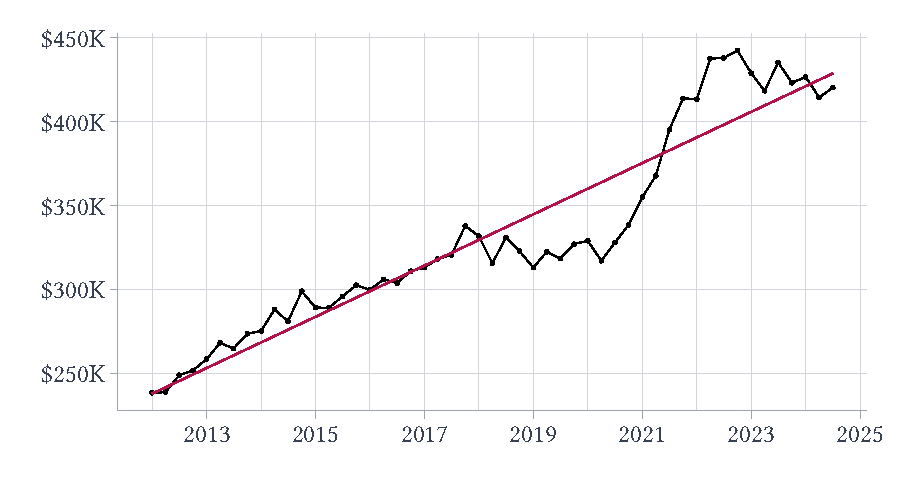
\includegraphics[width = 0.9\textwidth]{figures/median_us_housing_price_raw.pdf}
  \end{center}
\end{figure}

\begin{figure}[h!]
  \caption{Daily data on the Number of Taxis available at Noon in NYC}
  \label{fig:taxi}

  \vspace*{-\bigskipamount}
  \begin{center}
    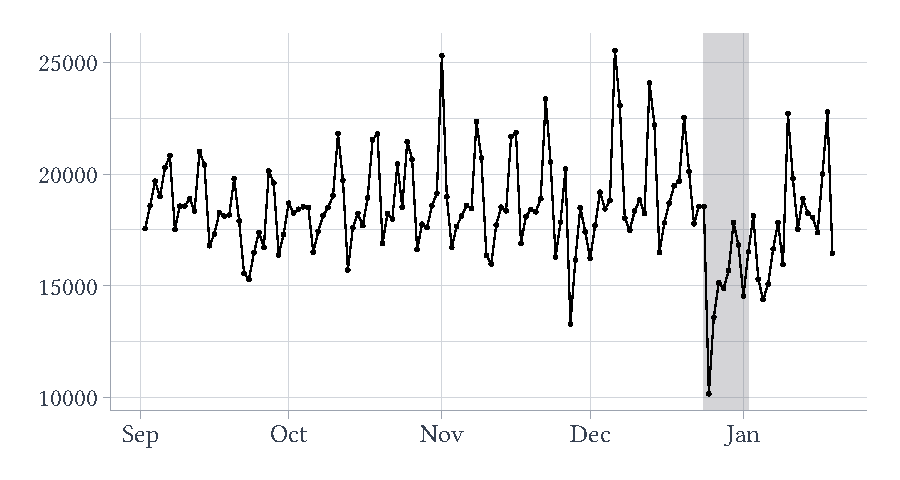
\includegraphics[width = 0.9\textwidth]{figures/nyc_taxis_raw.pdf}
  \end{center}
\end{figure}



\end{document}
